\documentclass[11pt,titlepage]{article}

\usepackage[american]{babel}
\usepackage[utf8]{inputenc}
\usepackage[T1]{fontenc}
\usepackage{lmodern}
\usepackage{amsmath,amsfonts,amssymb}
\usepackage{graphicx}
\usepackage{geometry}
\geometry{a4paper}
\usepackage[parfill]{parskip}
\usepackage{graphicx}
\usepackage{amssymb}
\usepackage{epstopdf}
\usepackage{color}
\usepackage[tt]{titlepic}
\usepackage{fancyhdr}
\usepackage{enumerate}
\usepackage{lastpage}
\usepackage{float}
\usepackage{amsmath}
\usepackage{amsfonts}
\usepackage{amsthm}
\usepackage{enumerate}
\usepackage{enumitem}
\usepackage{physics}
\usepackage{bm}
\usepackage{setspace}
\usepackage{mathtools}
\usepackage{subcaption}
\usepackage{relsize}
\usepackage{listings}
\usepackage{array}
\usepackage{caption}

% Custom Defines
\usepackage[comma,numbers,sort&compress]{natbib}
\bibliographystyle{plainnat}
\usepackage[pdfstartview=FitH,
            breaklinks=true,
            bookmarksopen=true,
            bookmarksnumbered=true,
            colorlinks=true,
            linkcolor=black,
            citecolor=black
            ]{hyperref}
\newcommand{\rmd}{\textrm{d}}
\newcommand{\bi}[1]{{\ensuremath{\boldsymbol{#1}}}}
\definecolor{gray}{rgb}{0.5,0.5,0.5}

\topmargin=-0.45in
\oddsidemargin=-0.1in
\textwidth=6.8in
\textheight=9.2in
\headheight=30.9pt

\renewcommand{\bibsection}{}
%======================= SET YOUR NAME HERE =======================================
\def\MyName{Matteo Calafà}

%======================= Titlepage (DO NOT MODIFY) ================================
\titlepic{
\includegraphics[width=5cm]{Figures/EPFL_LOGO.jpg}}
\title{\textbf{Report}\\Course Project: Statistics of Turbulence and the Onset of Chaos}

\author{~\\[3cm]~
\begin{tabular}{rl}
Name:&\MyName\\
Date:&\today\\
Course:&Turbulence ME-467\\
Instructor:&Tobias Schneider
\end{tabular}}
\date{}
%==================================================================================



\begin{document}
%========================  Header (DO NOT MODIFY) =================================
\pagestyle{fancy} \pagenumbering{arabic} \setcounter{page}{1}
\addtolength{\headheight}{\baselineskip}
\lhead{\textbf{ME-467: Turbulence}\\\MyName}
\chead{REPORT\\ \textit{Statistics of Turbulence and the Onset of Chaos}}
\rhead{
\includegraphics[width=55pt]{Figures/EPFL_LOGO.jpg}}
\rfoot{\vspace{5pt}{\fontfamily{phv}\fontsize{5}{5}\selectfont ME-467 Project 2022, \MyName{}, \the\day.\the\month.\the\year, \thepage/\pageref{LastPage}}}
\renewcommand{\headrulewidth}{0.4pt}
\maketitle
%==================================================================================

\section{Part I: Statistical Analysis of Turbulence}

\subsection{Introduction} % Remove limit text
The Kolmogorov theory gives us some results of the decaying rates of the main quantities in the case of unforced turbulence. Observing experimentally that turbulence decays slowly (i.e. with power and not exponential law), the theory is able to predict these power laws starting from some assumptions and a value for the fixed parameter $h$. These results are also later shown in section \ref{turbulence_decay}. \\
As anticipated, the theory requires some further assumptions since K41 hypotheses are not enough. First of all, it is assumed that the velocity associated to large scales has an \emph{infrared asymptotic self-similarity}, i.e. $v_l \sim Cl^h$ for $l \rightarrow \infty$ and a certain constant parameter $h$. Then, the \emph{Principle of Permance of Large Eddies} must hold: briefly, if $v_l$ has initially infrared asymptotic law with $-5/2 < h < -1$ and there is no external force, then it is expected to preserve this property in time. This is a non-trivial and not proved statement and it is clearly not included in the K41 theory. \\
This result implies the energy spectrum to have a $k^{-1-2h}$ law for $k\rightarrow 0$. However, to fit the physical results and the K41, it is needed to assume that there exists a length $l_0$ such that the above law is valid only for bigger length scales. On the other hand, the one provided by the $5/3$ law will be valid only for scales smaller than $l_0$ as indeed already stated in the K41 theory. \\
Another aspect that would cause inconsistencies with the standard K41 theory is the fact that these results lead to the temporal law of the integral length scale $l_0$ while the classical theory deals with stationary turbulence. However, this is justified by the fact that the power law decay is still very "slow" with respect to the internal turbulence time scales. \\
Moreover, the decay rates are achieved thanks to the initial hypothesis that $Re = l_0 v_0/\nu \gg 0$ in time. This is an important assumption to assure that turbulence is still effective at the length scale whatever the value of the length scale and instant of time. \\
To conclude, we remind again that these results are restricted only to homogeneous and isotropic flows, following the hypothesis of the Kolmogorov theory.


\subsection{Data Analysis}

\subsubsection{Velocity Signal in the Spatial Domain}\label{velocity_signal_in_the_spatial_domain}
The measurements correspond to streamwise velocities detected at a frequency $f=20kHz$. This implies that each measurement follows the previous one after 
\begin{equation} \label{eq1}
\Delta t = 1/f
\end{equation}
In this way, we can get the velocity measurements with respect to time. To instead plot them with respect to space, we exploit the Taylor frozen hypothesis to get the distance in space between two measurements as 
\begin{equation} \label{eq2}
	\Delta x \simeq - <u> \Delta t \overset{(\ref{eq1})}{=} -<u>/f
\end{equation}
	where $<u>$ is the mean velocity at each anemometer. \\ 
Our choice for the first plot (Fig. \ref{fig1}) was to take a maximum distance of 4 meters. With the above formulae, it is then easy to get the number of measurements to plot. It is just needed to pass from the distance in space to the distance in time and see the ratio with respect to $\Delta t$. These results are finally shown in Fig. \ref{fig1}. \\

	\begin{center}
	\begin{figure} [h]
		\centering
		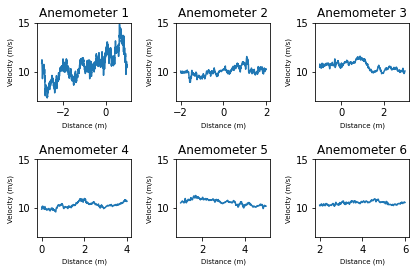
\includegraphics[width = 4.5in]{./figures/ex1_1.png}
		\caption{PLOT A - Streamvise velocity measurements for each anemometer. The plots are shown with respect to space thanks to the Taylor frozen hypothesis.}
		\label{fig1}
	\end{figure}
\end{center}

The $x$ values represent the spatial position of the anemometer and the previous $4m$ as in our choice. First of all, we notice that the mean velocity is almost constant for each anemometer ($\approx 10m/s$). This is expected because of conservation of mass and constant inlet velocity. I.e., the same quantity of air that goes inside the tunnel should goes outside at the same moment if the density is considered constant or almost constant. Because the velocity at the inlet is constant, it implies that the mean velocity should be approximately constant everywhere.

On the other hand, oscillations are more evident in the first anemometer and they later vanish. This is expected and due to two main reasons: the first one is due to the difference between the entrance/unstable region of the tunnel and the fully-developed region where the flow is more asymptotically stable. The second reason is instead related to the decay of unforced turbulence. Clearly, the only applied force is at the inlet of the tunnel where turbulence is therefore more intense. \\

In Table \ref{table1} we instead show the results of mean velocities and turbulence intensities. To obtain them, it is enough to compute respectively the mean and the normalized standard deviation of the velocities measurements at each anemometer. These results clearly confirm the previous discussion: the mean velocity is almost constant in each anemometer and turbulence intensities instead decrease. Clearly, turbulence intensities are related to the turbulence decay and the decrease of oscillations in Fig. \ref{fig1}.

\begin{table} [h]
\centering
\caption{Table of results 1.} \label{table1}
    \begin{tabular}{ | c | c | c | c | c | c | c | c |}
        \hline
        Param. & Dim. & $A_1$ & $A_2$ & $A_3$ & $A_4$ & $A_5$ & $A_6$ \\
        \hline
        $d$ & $m$ & 1.0 & 2.0 & 3.0 & 4.0 & 5.0 & 6.0 \\
        \hline
        $U$ & $m/s$&10.52223399 &10.52201583&10.52117473 &10.52232686& 10.52234804& 10.52185721 \\
        \hline
        $I$ & adim.& 0.12180673& 0.05480351& 0.03954964 &0.0320026  &0.02713776& 0.02407247 \\
        \hline
    \end{tabular}
\end{table}

Certainly, the Taylor frozen hypothesis is just an approximation of the real phenomenon since turbulence has a certain effect on the flow variations. In general, the approximation is valid if the turbulence intensity is very small but this is not our case (especially at the beginning where this values is more than $0.12$). Moreover, the turbulence intensity changes a lot in space and this gives incoherent results: see for instance in Fig. \ref{fig1} the velocity measurements in the second anemometer at the position $x=-2m$. This trend is completely different from velocity measured by the first anemometer and associated to the same spatial position. This is because we miss the measurements in the intermediate positions where turbulence intensities have inevitably different values. \\
However, the error in the estimation of intermediate velocity profiles can be easily bounded. The mean velocity is approximately the same in all the positions while the turbulence intensity can be achieved through an extrapolation. In particular, the turbulence intensity follows a trend similar to the ones presented in section \ref{turbulence_decay} (it is indeed equivalent to the square root of the kinetic energy except for a constant coefficient). Therefore, from the results in the table and the assumption of the trend, a regression analysis can be performed to estimate these values in all the intermediate positions.

\subsubsection{Correlation Length of the Velocity Signal} \label{correlation_length_of_the_velocity}
In table \ref{tab2} we show the measures of the correlation length and the integral scale. To compute the autocorrelation, we exploited the optimized \texttt{correlate} function from \texttt{Scipy}. To compute the integral scale, we used the same function and after a rectangular quadrature formula for the integral. First of all, we notice that the two scale lengths are very similar which confirms the fact that the first theoretically approximates the second.
\begin{table}[h]
\centering
\caption{Table of results 2.} \label{tab2}
    \begin{tabular}{ | c | c | c | c | c | c | c | c |}
    \hline
    Param. & Dim. & $A_1$ & $A_2$ & $A_3$ & $A_4$ & $A_5$ & $A_6$ \\
    \hline
    $L_C$ & m & 0.36669985& 0.63447755& 0.77330634& 0.90386788 &1.00909318 &1.08532957 \\
    \hline
    $L_\mathrm{int}$ &m & 0.35895344& 0.62704922& 0.76843644& 0.88769361 &1.00077964 &1.07598959 \\
    \hline
    \end{tabular}
\end{table}

In Fig. \ref{fig2}, we instead graphically show the trend of the correlation length.
	\begin{center} 
	\begin{figure} [h]
		\centering
		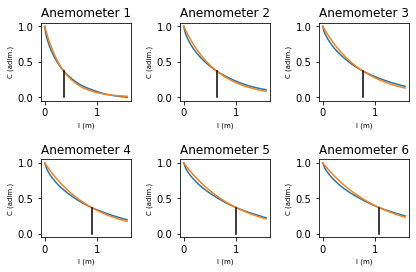
\includegraphics[width = 4.5in]{./figures/ex1_2.png}
		\caption{PLOT B - Correlation lengths with respect to the space distance $l$ (blue curves). Orange lines represent instead the functions $e^{-\frac{l}{L_C}}$. Finally, the black lines are the associated $L_C$ values.}
		\label{fig2}
	\end{figure}
\end{center}

Before discussing the trend of these lengths, let us clarify why the two are very similar. Giving a glance at the plots, we recognize soon an exponential decay of the correlation function. Since $C(0)=1$ always (by definition and also from the plots) we conclude that it is approximately in the form: $C(l) = e^{-al}$ for a certain steep coefficient a. It implies that:
\begin{equation*}
	L_{int} := \int_0^{\infty} C(l)\, dl =  \int_0^{\infty} e^{-al}\, dl = \frac{1}{a}
\end{equation*}
We now notice that $1/a$ is also the value such that $C(1/a) = e^{-1}$, from here it follows the equivalence of the two definitions of length scale. In addition, these exponential laws are added to Fig. \ref{fig2} to show the effective overlap of the autocorrelation function with its analytical approximation.\\

Let us now discuss the trend of the lengths. Intuitively, we can say that the decaying of turbulence implies a stronger correlation between distant points. In other words, when the turbulence is strong, the noisy dynamics implies the velocity vectors to be almost independent despite they might be close. \\ 
Another reason to convince us of this correct trend is the relation between these length scales and the integral length scale presented in section \ref{energy_spectrum}. We will show later the trend of the latter but we now anticipate that it will increase following the theoretical predictions. Therefore, $L_C$ and $L_{int}$ correctly increase as $l_0$ does.

\subsubsection{Energy Spectrum of the Flow} \label{energy_spectrum}
In Fig. \ref{fig3} we report the measured energy spectrum for each anemometer.
	\begin{center} 
	\begin{figure} [h]
		\centering
		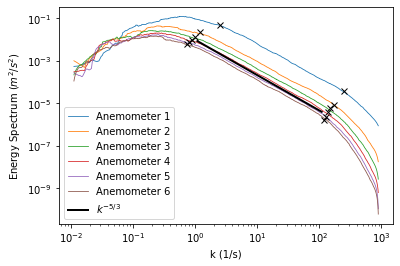
\includegraphics[width = 5in]{./figures/ex1_3.png}
		\caption{PLOT C - Log-log plot of the energy spectrum of the velocity measurements for each anemometer.  Also a black line that indicates the $-5/3$ slope has been inserted.}
		\label{fig3}
	\end{figure}
\end{center}

The energy spectrum has been calculated exploiting the optimized \texttt{fft} algorithm from \texttt{Scipy} for the positive frequencies and the inverse \texttt{ifft} for the negative frequencies. After that, it is just needed to sum the two contributions (as in the instructions, $E(k) = \tilde{E}(k) + \tilde{E}(-k) )$) paying attention to consider the correct multiplicative coefficient (i.e. $(\Delta x)^2$). As a confirmation, we report here the relative error between
\begin{equation*}
	\frac{1}{2}<u^2> \text{ and } \int_0^\infty E(k)\, dk
\end{equation*}
for the first anemometer that turns out to be: $2.47 \cdot 10^{-7}$. This very small value is due to the fact that the energy spectrum has been calculated very precisely using the full dataset (this is indeed possible in short times, i.e. less than one minute, thanks to the optimized functions cited above). \\
To conclude the implementation aspects, the original noisy spectrum has been later filtered with a \emph{Savitzky-Golay filter} (\cite{savgol}). More precisely, a standard application of the filter would overshoot in the left part of the plot because, in a log-log plot with originally equidistant $k$ values, the density of the number of points increases towards the right part of the plot. Therefore, a regression-based filter as Savitzky-Golay would be unbalanced in the two different regions. Our proposed solution is to interpolate the original spectrum at points that follow an exponential grow so that, in a log-log plot, they appear equi-distant and the filter can be then well-balanced. \\

We can finally comment the plots in Fig. \ref{fig3} and see how they respect the predictions of the Kolmogorov theory. We can indeed clearly distinguish the three regions (from left to right: the large scales with driving forces, the inertial range and the dissipation region with small scales). In particular, the inertial range clearly respects the $5/3$ law since the straight line is perfectly parallel to the trend of all the anemometers. Moreover, the large scales lines seem to respect the order predicted in the turbulence decay theory (indeed, this will be shown later in section \ref{turbulence_decay}). \\

From the energy spectrum, we can detect the starting and ending points of the inertial range that correspond to the integral and Kolmogorov frequencies. These points have been signed in the plot with black crosses. Finally, from these frequencies, we can get the integral and Kolmogorov length scales that are reported in table \ref{tab3}. \\

\begin{table}[h]
\centering
\caption{Table of results 3.}\label{tab3}
    \begin{tabular}{ | c | c | c | c | c | c | c | c |}
    \hline
    Param. & Dim. & $A_1$ & $A_2$ & $A_3$ & $A_4$ & $A_5$ & $A_6$ \\
    \hline
    $L_{\mathrm{int},E}$ & m &2.51327412 &5.23598776& 6.28318531& 6.98131701& 7.85398163 &8.37758041 \\
    \hline
    $\eta_E$ & m& 0.02513274 &0.03695991 &0.0418879&  0.0448799&  0.04833219& 0.05235988  \\
    \hline
    \end{tabular}
\end{table}
Reminding what has been discussed in section \ref{correlation_length_of_the_velocity} about the increase of the correlation length, also here the length scales increase with the distance $d$ because of the same reason as before. \\
As a last result, we want to check effectively the relationship between the two integral scales. This is shown in Fig. \ref{fig4}. Here, we show that the two scales are in fact approximately proportional. This fact should not surprise since turbulence length scales are known to be successfully represented by both autocorrelation and spectral length scales and therefore they must scale together (see for instance \cite{trush_2020}).\\
To conclude, we observe that every time $L_{int,E}$ and $\eta_E$ will be used to achieve new results, we will always incur in some inaccuracies due to the graphical detection of these values from the plot that, by its nature, is not precise.
	\begin{center} 
	\begin{figure} [h]
		\centering
		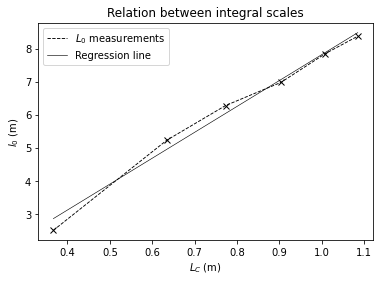
\includegraphics[width = 4in]{./figures/ex1_3_plus.png}
		\caption{EXTRA - Relation between the integral scale length and integral length of section \ref{correlation_length_of_the_velocity}. Despite some inaccuracies due to the rough $L_0$ detection on the plot in Fig. \ref{fig3}, the two values are clearly proportional.}
		\label{fig4}
	\end{figure}
\end{center}


\subsubsection{The Dissipation Rate and Different Reynolds Numbers}
In table \ref{tab4} we report the values for the energy dissipation rate, the Taylor Reynolds numbers and the Reynolds number that have been computed starting from the results of the previous sections. \\

\begin{table}[h!]
\centering
\caption{Table of results 4.} \label{tab4}
    \begin{tabular}{ | c | c | c | c | c | c | c | c |}
        \hline
        Param. & Dim. & $A_1$ & $A_2$ & $A_3$ & $A_4$ & $A_5$ & $A_6$ \\
        \hline
        $\epsilon$ & $m^2/s^3$&2.87076074& 0.15110392& 0.04658421& 0.02112303& 0.01153716 &0.00748596  \\
        \hline
        $Re_\lambda$ & Adim. & 969.527172 & 855.4148643& 802.221265 & 780.2180855& 759.1436670&
        741.4848821 \\
        \hline
        $Re$& Adim. &310190.581 & 290554.460& 253269.393 &227787.447&
        217626.8078 &204905.321 \\
        \hline
    \end{tabular}
\end{table}
We can again give both a physical interpretation and a mathematical explanation to the decreasing trend of $\epsilon$. First of all, as $\epsilon$ represents the rate of turbulent kinetic energy dissipated in thermal energy, it is clear that the decaying turbulence implies a lower rate of energy shift and then a lower dissipation rate for higher $d$. The second motivation is due to the fact that, by definition of $\epsilon$ and the previous relation between length scales, we can state that $\epsilon \sim E^{3/2}/l_0$. Using the rates from the turbulence decay theory (section \ref{turbulence_decay}, equations \ref{l_0_decay}, \ref{E_decay}), we can soon achieve an order of $2h/(1-h)$ for $\epsilon$ with respect to $d$, therefore a power decreasing law. \\
Comparing instead the Reynolds numbers, the decreasing trend is again expected from the theory of turbulence decay and, moreover, $Re_{\lambda}$ scales as the square root of $Re$ (except for a coefficient $\approx 2$) as predicted from K41. \\
To conclude, these trends are all coherent with the turbulence decay results and therefore also with the trend of $I$ from section \ref{velocity_signal_in_the_spatial_domain}.
\subsection{Turbulence Decay} \label{turbulence_decay}
In table \ref{tab5} we report the computations of the kinetic energies per unit mass. This is defined as $\mathcal{E} = 3/2<u^2>$ and the $3$ factor comes from the number of dimensions. Indeed: 
\begin{equation*}
	\mathcal{E} = \frac{1}{2} < \vec{u} \cdot \vec{u} >= \frac{1}{2} < u_x^2 + u_y^2 + u_z^2 > = \frac{3}{2} <u^2>
\end{equation*}
Where the last equality comes from an isotropic assumption. Indeed, what we measure is the streamwise velocity $u_x$ that is assumed to be equal also in the other directions.
\begin{table}[h!]
\centering
\caption{Table of results 5.} \label{tab5}
    \begin{tabular}{ | c | c | c | c | c | c | c | c |}
        \hline
        Param. & Dim. & $A_1$ & $A_2$ & $A_3$ & $A_4$ & $A_5$ & $A_6$ \\
        \hline
        $\mathcal{E}$&$m^2/s^2$ &2.46405129& 0.49877643& 0.25971965& 0.1700926 & 0.12231075 &0.09623149  \\
        \hline
    \end{tabular}
\end{table}

We finally report the laws predicted from the theory of turbulence decay:
\begin{equation} \label{l_0_decay}
	l_0 \propto (d-d_0)^{1/(1-h)}
\end{equation}
\begin{equation}\label{u_0_decay}
	u_0 \propto (d-d_0)^{h/(1-h)}
\end{equation}
\begin{equation}\label{Re_decay}
	Re \propto (d-d_0)^{(1+h)/(1-h)}
\end{equation}
\begin{equation}\label{E_decay}
	E \propto (d-d_0)^{2h/(1-h)}
\end{equation}
Where $d_0$ and $h$ are constants. We will equivalently analyse $\mathcal{E}$ instead of $E$.
	\begin{center} 
	\begin{figure} [h]
		\centering
		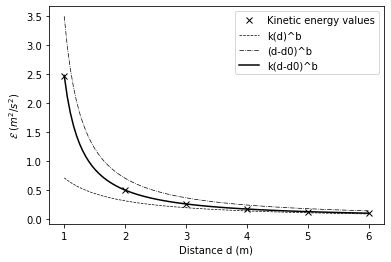
\includegraphics[width = 4in]{./figures/ex1_5_1.png}
		\caption{EXTRA - Fitting of the turbulence kinetic energy per unit mass. The other dashed lines are just to show the importance of both $k$ and $d_0$ parameters.}
		\label{fig5}
	\end{figure}
\end{center}
\paragraph{First method:}
The first objective is to find $d_0$ and $h$ from the measurements of $\mathcal{E}$ through a fitting method. Certainly linear regression cannot be used because of the non linearity of the exponent, however we can notice that:
\begin{equation}\label{log_eq}
	\exists K, d_0, b \hspace{3mm} \text{ such that } \hspace{3mm} \mathcal{E}(d) \approx K(d-d_0)^b \hspace{3mm} \Leftrightarrow \hspace{3mm} \ln{\mathcal{E}} \approx \ln{K} + b \ln{(d-d_0)}
\end{equation}
Therefore, applying the logarithm to the data, we only have one non-linear coefficient that is $d_0$. The proposed algorithm is then the following: 
\begin{enumerate}
	\item We iterate over a set of hypothetical values for $d_0$ (numerous enough).
	\item For each of these, we compute the optimal $K$ and $b$ through linear regression.
	\item Given the choice of $d_0,K,b$, we compute the resulting MSE error.
	\item At the end of the loop, we take the $d_0$ that gave the lowest MSE error.
	\item We can finally get the associated $K$ and $b$ again from linear regression.
\end{enumerate}
	This is a simple and quick algorithm since iterations are performed over only one parameter. The resulting values are then: $d_0 \simeq 0.65$, $h \simeq -1.46$. In addition we show in Fig. \ref{fig5} the successful fitting method. From now on,  for simplicity, we will consider the optimal exponent as $h=-1.5 = -3/2$. 

\paragraph{Second method:}
Taking again equation \ref{log_eq}, we then have proven that for correct values of $d_0,b,K$ the log-log plot of $\mathcal{E}$ against $d$ is approximately a straight line. Fig. \ref{fig6} shows a  log-log plot of $\mathcal{E}$ against $(d-d_0)$ for different values of $d_0$. For the same reason as before, only the correct $d_0$ generates a straight line. Indeed, only the pink and grey lines are close to be straight, therefore $d_0$ is between 0.6 and 0.7 as confirmed by the fitting method. Taking it in the middle ($=0.65$), we can estimate $q$ looking at the slope of the lines. The black line shows the trend of $\mathcal{E}$ predicted by choosing the previous value for $d_0$ and the correct $q$ to have parallel lines. Looking at the numerical values of $d_0$ and $q$, we conclude that the graphical and fitting methods are coherent. Indeed, for both, the correct shifting parameter is approximately $d_0=0.65$ and the exponent $h=-3/2 \Leftrightarrow q = -6/5$. 

	\begin{center} 
	\begin{figure} [h]
		\centering
		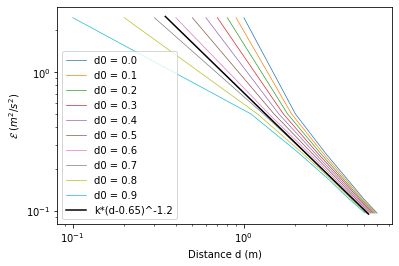
\includegraphics[width = 4in]{./figures/ex1_5_2.png}
		\caption{PLOT D - Log-log plot of the measured $\mathcal{E}$ with respect to $(d-d_0)$ for different $d_0$. As explained in equation \ref{log_eq}, only the correct $d_0$ generates a straight line. Therefore, the correct $d_0$ is between 0.6 and 0.7. Hence, we have chosen $d_0=0.65$.  After that, the exponent $q$ has been chosen such that the line has the same slope. Finally, the graphical method prediction is shown through the black line.}
		\label{fig6}
	\end{figure}
\end{center}


\paragraph{Third method:}
Another confirmation comes from the scaling property:
\begin{equation}\label{eq_E_L0}
	\mathcal{E} \propto l_0^{2h}
\end{equation}
First of all, we inform that we can replace $l_0$ with $L_C$ thanks to the reasons given at the end of section \ref{energy_spectrum}. Therefore, we aim now to study this relation and a comparison between the experimental values of $\mathcal{E}$ against $L_C$ is shown in Fig. \ref{fig7}. 

	\begin{center} 
	\begin{figure} [h!]
		\centering
		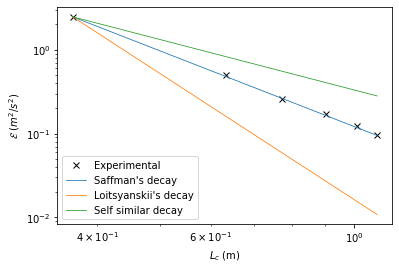
\includegraphics[width = 4in]{./figures/ex1_5_3.png}
		\caption{PLOT E - Log-log plot of the measured $\mathcal{E}$ with respect to $L_C$.}
		\label{fig7}
	\end{figure}
\end{center}

The power law of $\mathcal{E}$ is evident from the straightness of the line. Moreover, these measures coincide almost exactly with the ones from the \emph{Saffman's decay} under which $h=-3/2$. This is expected since we have already shown from the previous methods that $h$ is approximately $-1.5$. \\
Seeing the excellent overlapping of the experimental values with the Saffman's decay predictions, it should not surprise that the fitting method applied  to equation \ref{eq_E_L0} with fixed $h=-1.5$ returns again a parameter $d_0$ that is approximately $0.65$. 

\paragraph{Comparison of the methods:}
To conclude this part about the estimation of $d_0$ and $h$, we can observe that the three methods are indeed equivalent since they return the same values (except for approximations). Advantages and disadvantages of each one are listed below:
\begin{itemize}
	\item The fitting method is very precise. However, it can be a bit slower if compared to the others because of the several calculations (even if it is in general quite fast). In addition, it is harder to interpret results only from the numerical values.
	\item The graphical method is instead good to interpret results. However, it is not precise at all. 
	\item The relation with $L_0$ is precise and has theoretical supports. However, it restricts to only 3 possible theories and it is computationally slow as the first method (since it still needs to iterate over $d_0$).
\end{itemize}

\paragraph{Turbulence decay and energy spectrum: } 
 In Fig. \ref{fig8} we show again the energy spectrum. This time we want to study it with respect to the prediction of its trend for large eddies. Despite some noise (we have already discussed the issue of a fitting/filtering method in a logaritmic scale, see section \ref{energy_spectrum}), the lines seem parallel to the predicted line. Therefore, our theoretical results and the choice of $h=-3/2$ seem to confirm again the experiments.
 
 	\begin{center} 
 	\begin{figure} [h]
 		\centering
 		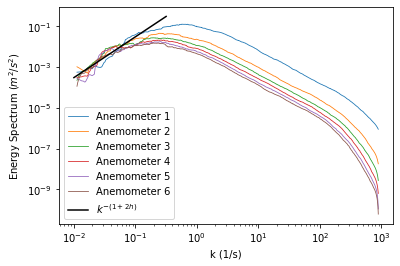
\includegraphics[width = 4in]{./figures/ex1_5_4.png}
 		\caption{PLOT F - Energy spectrum (already shown in Fig. \ref{fig3}) with the theoretical trend for the large scales. Despite some noise, the spectrum seems to scale as the predicted trend.}
 		\label{fig8}
 	\end{figure}
 \end{center}

\paragraph{Discussion about the virtual origin $d_0$:}
The virtual origin $d_0$ is certainly not only a fitting parameter but represents, in a certain way, the starting positions for the decaying turbulence predicted trends. In other words, the laws in equations \ref{l_0_decay}, \ref{u_0_decay}, \ref{Re_decay}, \ref{E_decay} do not have any validity for distances $d < d_0$, neither mathematically (exponentials of negative bases) nor physically. Until the distance $d_0$, the turbulence is expected not to freely decay but, instead, to be still forced. This is the reason why our $d_0$ value is between $0m$ and $1m$, i.e. in the inlet region where applied forces have still a dominant role in the turbulence process. \\
We expect $d_0$ to be approximately the same for all the above relations (eq. \ref{l_0_decay}, \ref{u_0_decay}, \ref{Re_decay}, \ref{E_decay}) since, the condition of forced/unforced turbulence should hold independently for all the above quantities. Moreover, mathematically, the cited relations are all achieved from one of those and therefore the $d_0$ is the same for each one. However, these are scaling relations and there are inaccuracies in the values achieved for $l_0$ and $Re$, so we do not expect to achieve experimentally the exact same value of $d_0$ for all these quantities. We have indeed performed some fitting methods on equations \ref{l_0_decay} and \ref{Re_decay} fixing the exponent $h=-3/2$ and we achieved respectively $d_0 = 0.75m$ and $d_0 = 0.25m$. Despite these values are not similar with the previous $d_0 = 0.65m$, we still have values in the same interval $0m-1m$ to confirm our theoretical predictions. In addition, we show in Fig. \ref{fig9} that the choice for the $h$ value is suitable also for the $l_0$ and $Re$ values.



\begin{center}
	\begin{figure} [h]
		\centering
		\subfloat[Fitting for $l_0$ values]{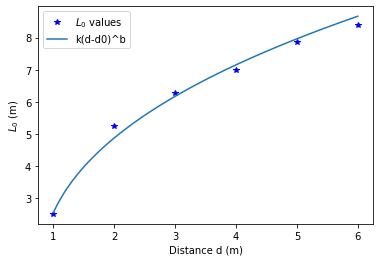
\includegraphics[width = 2.7in]{./figures/ex1_5_5.png}} 
		\hspace{8mm}
		\subfloat[Fitting for $Re$ values]{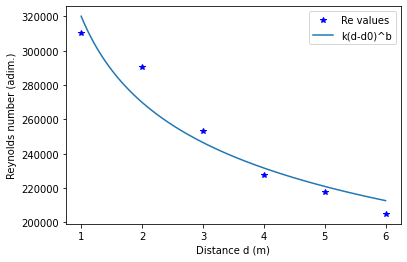
\includegraphics[width = 2.9in]{./figures/ex1_5_6.png}}
		\caption{EXTRA - Fitting method applied to equations \ref{l_0_decay} and \ref{Re_decay} fixing $h=-3/2$. We clearly see that this value for $h$ is well suitable also for these quantities.}
		\label{fig9}
	\end{figure}
\end{center}

\subsubsection{Velocity Increments}
In Fig. \ref{fig10} we show the behaviour of the longitudinal velocity increment $\delta v_{||}(x,l):=u(x+l)-u(x)$ for the distances $l=\{1mm, 1cm, 10cm, 10m\}$. 
\begin{center}
	\begin{figure} [h]
		\centering
		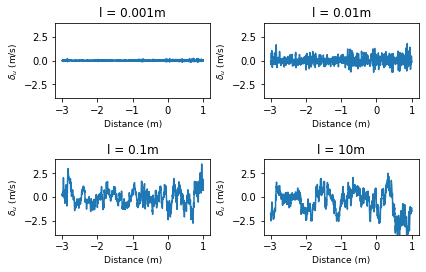
\includegraphics[width = 4in]{./figures/ex1_6.png}
		\caption{PLOT G - Longitudinal velocity increment for different distances $l$ and measured at the first anemometer.}
		\label{fig10}
	\end{figure}
\end{center}

First of all, considering the turbulent length scales in table \ref{tab3}, we can state that:
\begin{itemize}
	\item $l=1mm$ is in the dissipative region ($l<\eta_E$).
	\item $l=0.01m$ is between the dissipative and inertial region ($I \approx \eta_E$).
	\item $l=0.1m$ is in the inertial range ($\eta_E < l < L_{int,E}$).
	\item $l=10m$ is in the large scales region ($l > L_{int,E}$) even if the two lengths are quite comparable.
\end{itemize}

Focusing now on the results from Fig. \ref{fig10}, the behaviour is expected since a small $l$ implies strong similarity between the two measures (that are indeed near in space) where instead a big $l$ implies no connection and therefore a completely random difference. It is important to notice that this increment of randomness has a limit since two measures that are very distant in space are completely uncorrelated and so they show the same pattern whatever is the value of $l\gg0$. As a demonstration, the difference between the case with $l=0.1m$ and $l=10m$ is not so relevant if compared to the upper plots. \\
We conclude reminding that this kind of reasoning is very similar to the one made for the autocorrelation functions in section \ref{correlation_length_of_the_velocity}. In both cases, the increase of distance implies a decrease of correlation. \\
To further investigate the properties of $\delta u_{||}$ we might wonder whether this has a normal distribution. To do that, we analyse the trend of the flatness that is defined as:
\begin{equation*}
	f(l) := \frac{\left<\delta u_{||}^4(x,l)\right>}{{\left<\delta u_{||}^2(x,l)\right>}^2}
\end{equation*}
For a centred normal distribution, the fourth moment is known to be equal to $3\sigma^4$ while the second moment is the variance. Therefore the flatness is $3\sigma^4/(\sigma^2)^2 = 3$. The flatness of $\delta u_{||}$ is instead shown in Fig. \ref{fig11}

\begin{center}
	\begin{figure} [h]
		\centering
		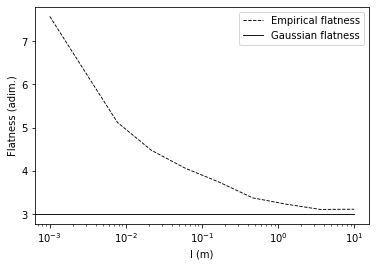
\includegraphics[width = 4in]{./figures/ex1_6_1.png}
		\caption{PLOT H - Longitudinal velocity increment flatness for different $l$. It is easy to see the convergence towards the normal flatness 3.}
		\label{fig11}
	\end{figure}
\end{center}
It is reasonable that the flatness tends to the one from the normal distribution because, as we stated above, big distances imply differences of independent measures and, hence, normally distributed. \\
The reason why the flatness is higher for small distances must be associated to the not normality of $\delta u_{||}(x,l)$ for small $l$. In particular, higher flatnesses are characteristic of the so-called \emph{leptokurtic} distributions, i.e. distributions that are more squeezed at zero and with fatter tails. An equivalent interpretation is the presence of more \emph{outliers}. Therefore, we can reasonably think of $\delta u_{||}$ for small $l$ as more concentrated in zero (see indeed Fig. \ref{fig10}) where, however, there are many outliers due to noisy turbulent effects. Physically, the difference between two near measures is usually small because of the high correlation, however, some noisy sudden effects can sometimes cause completely different measures.

\subsubsection{Structure Functions and Energy Dissipation}
In Fig. \ref{fig12} and  \ref{fig13} we show the trend of $S_2(l)$ and $S_3(l)$. We know from the K41 that the 5/3 law for the energy spectrum is related to the 2/3 law of $S_2$ (more precisely, from the latter we can obtain the former with the Wiener formula). First of all, we note that $S_2$ successfully satisfies the 2/3 law in a certain range. We would like to investigate now whether this is the same range of validity of the 5/3 law in Fig. \ref{fig3}. Since these plots are referred to only the first anemometer, we already computed the Kolmorov and integral length scale for the first anemometers as $\eta_E \approx 0.025m$ and $L_{int,E} \approx 2.51m$ (table \ref{tab3}). In this case, however, the clear $2/3$ slope is observed only in a smaller range where the lower bound is bigger than $0.01m$ and the upper bound is smaller than $1m$. Even if this range is shorter, it is centred (not shifted) as the one from the energy spectrum and has more or less the same order of magnitude. \\
The same could be noticed in Fig. \ref{fig13} for $S_3$ which respects the 4/5 law for a certain range that, also in this case, is similar but shorter than the one from the energy spectrum. To conclude, the trends of $S_2$ and $S_3$ support the K41 except these intervals should correspond to the one from $E(k)$. \\

\begin{center}
	\begin{figure} [h]
		\centering
		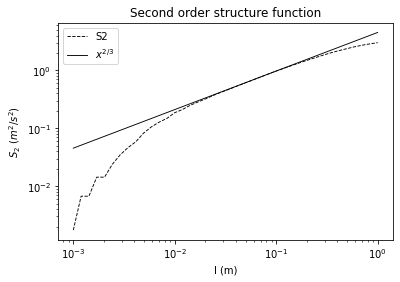
\includegraphics[width = 4in]{./figures/ex1_7_1.png}
		\caption{PLOT I - Second order structure function against distance $l$. In addition, the theoretical trend from K41.}
		\label{fig12}
	\end{figure}
\end{center}
A last notice is about the fact that from $S_2$ and $S_3$ we could potentially achieve a value for the energy dissipation rate $\epsilon$. Indeed the $2/3$ and $4/5$ laws state that:
\begin{equation} \label{S2_epsilon}
	S_2(l) = C_2 \epsilon^\frac{2}{3} l^\frac{2}{3} \hspace{4mm} \text{and} \hspace{4mm}S_3(l) = C_3 \epsilon l
\end{equation}
where $C_3 = -4/5$ and $C_2$ can be assumed to be $2.2$. Taking a value for $l$ that is valid for these laws (e.g. $l=0.07m$ is in the middle of the validity ranges in Fig. \ref{fig12} and \ref{fig13}) we can then use the inverses of the equations \ref{S2_epsilon} to get $\epsilon$. These calculations give indeed $\epsilon \approx 2.97 m^2/s^3$ from $S_2$ and $\epsilon \approx 3.01 m^2/s^3$ from $S_3$. These are satisfying results since the original value for $\epsilon$ was $approx 2.87 m^2/s^3$ (table \ref{tab4}).
\begin{center}
	\begin{figure} [h]
		\centering
		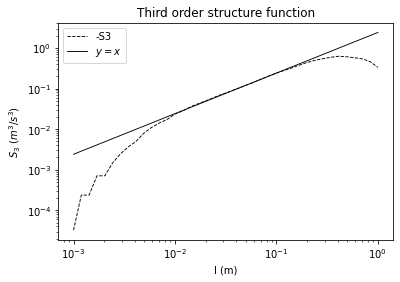
\includegraphics[width = 4in]{./figures/ex1_7_2.png}
		\caption{PLOT J - Third order structure function against distance $l$. In addition, the theoretical trend from K41.}
		\label{fig13}
	\end{figure}
\end{center}

\subsection{Discussion \textcolor{blue}{(Limit: 1 page)}} % Remove limit text

%==================================================================================
\newpage
\section{Part II: Nonlinear Dynamics and the Emergence of Chaos}


\subsection{Introduction \textcolor{blue}{(Limit: 1/2 page)}} % Remove limit text
\subsection{Analysis of the Dynamics}
\subsubsection{Implementation of the Map and (Numerical) Observations}
\subsubsection{Strange Attractor and Fractal Dimensions}
\subsubsection{Chaos and Lyapunov Exponents}
\subsection{Discussion \textcolor{blue}{(Limit: 1/2 page)}} % Remove limit text





\clearpage
\appendix
\section*{Appendix}
\subsection*{List of Sources}
\bibliography{sources}
\subsection*{List of Collaborators}

%========================  Personal Statement (DO NOT MODIFY) =====================
\subsection*{Personal Statement}
I hereby certify that I fully respect the stated Honor Code and specifically that:
\begin{enumerate}
\item My report is my original work prepared solely by me;
\item All sources used are cited;
\item All people I collaborated with are listed.
\end{enumerate}
		
\vspace{4em}
\begin{tabular}{ll}
\makebox[2.5in]{\hrulefill} & \makebox[2in]{\hrulefill}\\
\small{Signature (\MyName)} & \small{Date}
\end{tabular}
%==================================================================================

\end{document}